\documentclass[tikz,border=10pt]{standalone}
\begin{document}

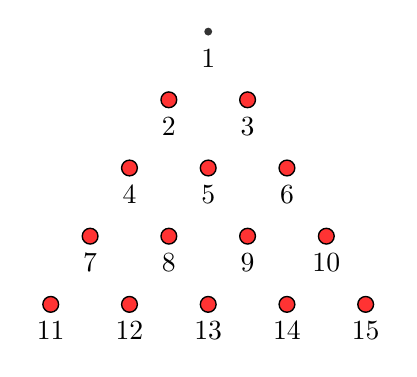
\begin{tikzpicture}

\tikzset{mycircle/.style={fill=red!80!white, draw=black, line width=0.5pt}}
\tikzset{mynode/.style={anchor=north, yshift = -0.1cm, text=black}}

\fill[black!80!white] (0,0) circle (0.05cm) node[mynode] {$1$};
\filldraw[mycircle] (-0.5, -0.866) circle (0.1cm) node[mynode] {$2$};
\filldraw[mycircle] (0.5,-0.866) circle (0.1cm) node[mynode] {$3$};
\filldraw[mycircle] (-1,-1.732) circle (0.1cm) node[mynode] {$4$};
\filldraw[mycircle] (0,-1.732) circle (0.1cm) node[mynode] {$5$};
\filldraw[mycircle] (1,-1.732) circle (0.1cm) node[mynode] {$6$};
\filldraw[mycircle] (-1.5,-2.598) circle (0.1cm) node[mynode] {$7$};
\filldraw[mycircle] (-0.5,-2.598) circle (0.1cm) node[mynode] {$8$};
\filldraw[mycircle] (0.5,-2.598) circle (0.1cm) node[mynode] {$9$};
\filldraw[mycircle] (1.5,-2.598) circle (0.1cm) node[mynode] {$10$};
\filldraw[mycircle] (-2,-3.464) circle (0.1cm) node[mynode] {$11$};
\filldraw[mycircle] (-1,-3.464) circle (0.1cm) node[mynode] {$12$};
\filldraw[mycircle] (0,-3.464) circle (0.1cm) node[mynode] {$13$};
\filldraw[mycircle] (1,-3.464) circle (0.1cm) node[mynode] {$14$};
\filldraw[mycircle] (2,-3.464) circle (0.1cm) node[mynode] {$15$};

\end{tikzpicture}

\end{document}